\subsection{Módulo Detector}
	\label{sec:detector}
	
	El módulo \textit{detector} (ver Figura \ref{fig:GeneralSystem}) es el encargado de detectar el inicio y final de cada trama. Esto lo hace a partir de validar que el contenido de la misma tenga N caracteres, conforme al formato de trama expuesto en la Sección \ref{sec:UART}. A medida que la validación tiene lugar, los caracteres ASCII son convertidos en valores booleanos (\textit{std\_logic}) dentro de un vector de elementos booleanos llamado \textit{packet}[N] (\textit{std\_logic\_vector} de N elementos). El diagrama de bloques de la máquina de estados finitos con camino de datos se muestra en la Figura \ref{fig:Detector_module}.
	
	\begin{figure}[H]
		\centering
		\includegraphics[width=1\textwidth]{Figuras/Detector_module.png}
		\centering\caption{FSMD del módulo \textit{Detector}.}
		\label{fig:Detector_module}
	\end{figure}
	
	En cada pulso de reloj (\textit{clk\_i}), el módulo UART envía un caracter por medio de la señal \textit{r\_data} (8 bytes) y un pulso (\textit{r\_available}) para informar que un nuevo dato ha sido enviado. El pulso de reloj es utilizado principalmente en el módulo \textit{Counter\_0\_to\_N}, cuyo parámetro N ya ha sido calculado por el ACG previo a generar el código y es la cantidad de caracteres que serán enviados a continuación del caracter de inicio. El proceso de detección y validación de la trama recibida se describe el diagrama de estados de la Figura \ref{fig:Detector_FSMD}.
	
	\begin{figure}[H]
		\centering
		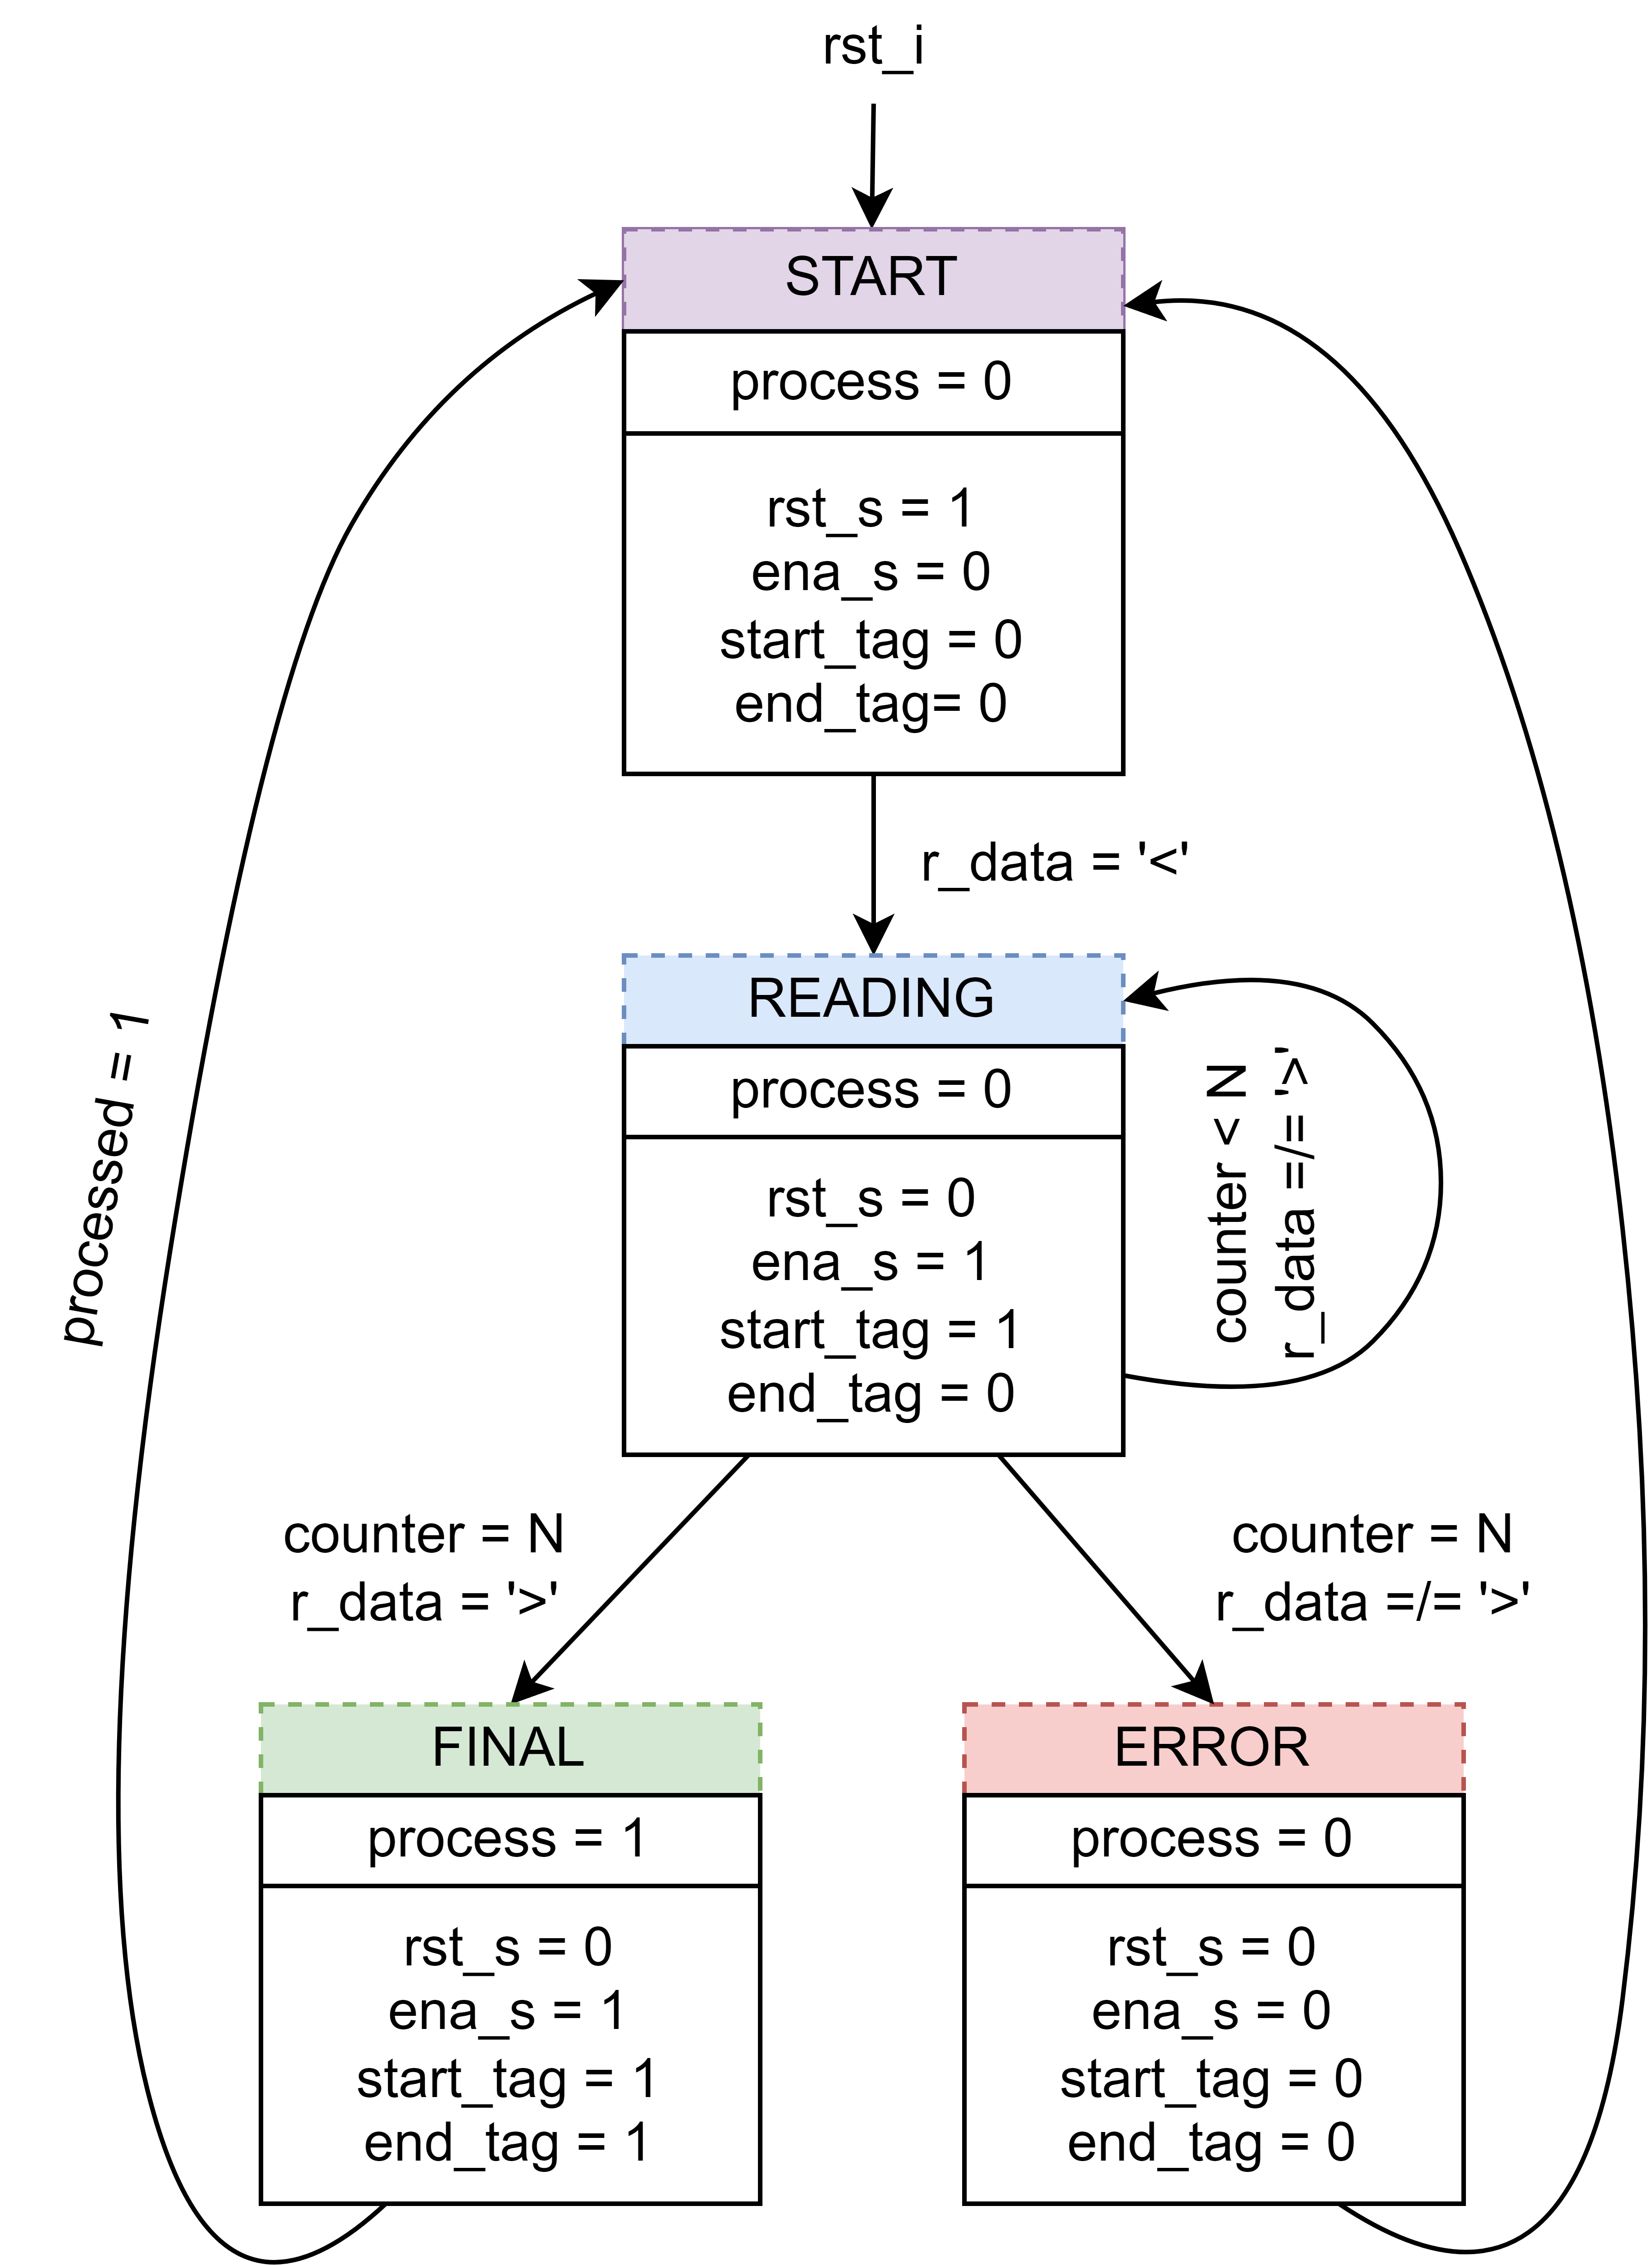
\includegraphics[width=0.8\textwidth]{Figuras/Detector_FSMD.png}
		\centering\caption{Diagrama de estados del módulo \textit{Detector}.}
		\label{fig:Detector_FSMD}
	\end{figure}
	
	El módulo \textit{Detector} inicia por detecto en el estado \textit{start}, aguardando por el caracter de inicio de trama '$<$'. Al recibir el caracter de inicio de trama, el módulo transiciona al estado \textit{reading}. En el estado \textit{reading} se recibirán solamente los caracteres hexadecimales '0' a 'F'. Si al terminar de recibir N caracteres, el próximo caracter no es el de fin de trama '$>$' entonces se transiciona al estado \textit{error}, se reinician las variables auxiliares, la trama se descarta y se vuelve al estado \textit{start}.
	
	Si el próximo caracter luego de leer N valores hexadecimales '0' a 'F' es el caracter de fin de trama '$>$', entonces el módulo transiciona al estado \textit{final}, donde se da por válida la trama y se habilita su envío al módulo \textit{decoder}, para volver al estado \textit{start} a la espera de un nuevo caracter de inicio de trama, y se reinician todas las variables auxiliares.
	
	Internamente se tienen diversas variables auxiliares para controlar si se han recibido los delimitadores y si la cantidad recibida es correcta. Eso cobra gran importancia al realizar los ensayos, porque se puede determinar rápidamente la fuente de eventuales errores.